\section{Structure et organisation des génomes procaryotes}
\label{sec:structure_org}

\subsection{Composants du génome : séquences codantes et non codantes}
\label{sec:gene}

Le génome se divise en 2 catégories : les séquences codantes, représentant la majorité du génome (entre 85 et 90 \%), et les séquences non codantes. Les séquences codantes sont divisées en unités appelées gènes. Les gènes jouent un rôle essentiel puisqu’ils contiennent l’information nécessaire à la production des protéines, impliquées dans toutes les réactions cellulaires. Ils renferment également les séquences pour produire des ARN ribosomiques (ARNr) et des ARN de transfert (ARNt), indispensables à la production des protéines (cf. \autoref{sec:fn_reg}).

Dans le génome, les gènes ne sont pas répartis aléatoirement. Ceux qui sont impliqués dans un même processus biologique sont souvent regroupés dans un contexte génomique. La conservation de l'ordre des gènes, appelée aussi synténie, peut varier entre les génomes, mais les gènes restent dans le même contexte \cite{lathe_gene_2000}, on parle alors de contexte conservé ou de synténie conservée. De plus, la position des gènes par rapport à l'origine de réplication (Ori: région où commence la réplication de l'ADN) a aussi son importance. Il a été montré que chez les bactéries avec un fort taux de division, les gènes ayant un rôle essentiel sont plus proches de l'Ori afin d'être plus fortement exprimés \cite{sharp_chromosomal_1989,vieira-silva_systemic_2010}.

Pour finir, les gènes peuvent être classés selon l’importance de leur fonction pour la survie de la cellule. Les gènes indispensables au cycle de vie d'une cellule, par exemple la réplication de l’ADN, la transcription, ou la traduction, sont dits "essentiels" et se distinguent des gènes "accessoires", qui codent pour des fonctions d'adaptation à des conditions particulières, comme la résistance aux antibiotiques, la défense contre les virus ou des réactions métaboliques spécifiques à une condition environnementale.

\begin{figure}[htbp]
    \centering
    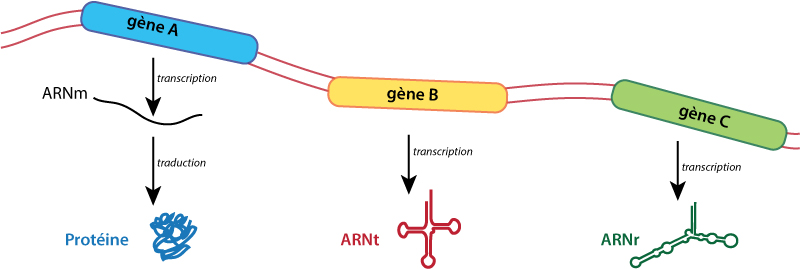
\includegraphics[width=\linewidth]{images/gene2prot.jpg}
    \caption[Représentation des gènes et de leurs produits]{\textbf{Représentation des gènes et de leurs produits : protéines et ARN.} Un gène est d'abord transcrit en ARN. Si l'ARN transcrit est dit messager (ARNm), il sera ensuite traduit en protéine, sinon l'ARN produit (ARNt ou ARNr) aura un rôle spécifique dans des processus cellulaires. Copié de RNBio, Sorbonne université. \url{https://rnbio.sorbonne-universite.fr/genetique_genotype1}}
    \label{fig:gene2prod}
\end{figure}

L'ADN non codant constitue une part tout de même non négligeable du génome et selon l'adage "la nature a horreur du vide"\footnote{Citation d'Aristote qui, répondant à Démocrite, rejetait l’idée du vide dans l’univers. On sait aujourd'hui que Démocrite avait raison, mais dans le cas des génomes procaryote, l'idée fonctionne.}. Il n'est donc pas inutile et renferme des fonctions essentielles à la vie de la cellule, comme les microARN et les ARN interférents (miARN et siARN). Ces ARN sont aujourd'hui considérés comme des acteurs clés dans la régulation des fonctions biologiques \cite{backofen_bioinformatics_2014,watkins_regulatory_2019}, mais aussi dans d'autres processus comme le système immunitaire \cite{bobadilla_ugarte_argonaute_2023}.

L'ADN non codant n'a pas uniquement le rôle de contenir les séquences transcrites en ARN, il contient aussi d'autres éléments régulateurs de l'expression des gènes contenus dans l'espace intergénique (cf. \autoref{sec:fn_reg}). On retrouve aussi dans l'ADN non codant des séquences répétées, en bordure des séquences d'insertion (IS) (qui se déplacent dans le génome), ou dans les séquences CRISPR (Régions composées de répétitions palindromiques, régulièrement séparées par des séquences appelées \textit{spacers}, impliquées dans le système immunitaire adaptatif des bactéries) \cite{jansen_identification_2002,bolotin_clustered_2005}. Il existe tout de même une partie d'ADN non codant qui n'a aucun rôle, ces séquences peuvent faire partie de l'espace intergénique, ou être des vestiges d'anciens gènes qui, au cours de l'évolution, ont perdu leur fonction (cf. \autoref{sec:dyn_evo}). Pour terminer, c'est aussi dans le non codant que l'on va retrouver des éléments essentiels dans la réplication et l'évolution des génomes procaryotes, comme l'origine de réplication (Ori).

\subsection{Réplicons et mécanismes de réplication dans les génomes procaryotes}
\label{sec:replicons}
Le terme réplicon désigne l’ensemble des molécules d’ADN capables de se répliquer de façon autonome. Un réplicon contient ainsi tous les éléments nécessaires à l’exécution et à la régulation de la réplication. Une cellule va contenir au moins un réplicon, mais elle en contient souvent plus. Les réplicons sont souvent circulaires, mais ils peuvent aussi être linéaires.

La forme de réplicon qui est toujours présente dans la cellule est le chromosome. Le chromosome, souvent circulaire et replié, constitue le plus grand réplicon en termes de paires de bases\footnote{La taille d’une séquence ou d’un génome se mesure en bases (b) ou paires de bases (pb).}. Une cellule peut contenir plusieurs chromosomes, dans ce cas, le plus grand sera considéré comme le chromosome principal et les autres comme secondaires. Par exemple, chez \textit{Rhodobacter sphaeroides}\footnote{Bactérie présente dans les lacs profonds et les eaux stagnants. Capable de réaliser la photosynthèse et avec un métabolisme versatile, elle est largement utilisée en biotechnologie} et \textit{Vibrio cholerae}\footnote{ Bactérie à l’origine du choléra, présente dans l’eau et transmissible entre humains, notamment via la transpiration.}, un second chromosome a été identifié \cite{suwanto_physical_1989,trucksis_vibrio_1998}.
\newpage
Une seconde forme de réplicon, connue pour son rôle dans l’évolution (voir \autoref{sec:evo_hz}), est le plasmide \cite{lederberg_gene_1946,lederberg_sex_1953}. Les plasmides sont souvent circulaires et de petite taille (par rapport au chromosome). Bien que certains plasmides puissent coder leurs propres protéines de réplication, et donc répondent à la définition de réplicon, ils peuvent dépendre de la machinerie de la cellule pour se répliquer. Quoi qu'il en soit, la réplication est indépendante du chromosome, ce qui leur permet d'être présents sous un grand nombre de copies. L’origine de réplication des plasmides diffère de celle des chromosomes. Elles sont généralement plus courtes et spécifiques, tandis que celle du chromosome est plus complexe et conservée. Par ailleurs, les plasmides peuvent accumuler de nouvelles séquences et augmenter en taille, prenant alors la forme de mégaplasmides (\autoref{fig:replicon}).

Chez la majorité des procaryotes, le chromosome contient les gènes essentiels, tandis que les plasmides portent des gènes accessoires. Cependant, certaines formes de réplicons oscillent entre chromosome et plasmide, que ce soit en termes de taille ou de contenu en gène. Le chromide \cite{harrison_introducing_2010} est une de ces formes. Sa taille est intermédiaire entre un plasmide et un chromosome principal, et il peut contenir des gènes essentiels à la cellule. Ces gènes présentent une proximité phylogénétique avec les espèces du même genre, contrairement à ceux du chromosome principal, qui sont conservés au-delà du genre. En revanche, en termes de mécanismes de réplication et de séquences Ori, les chromides utilisent des systèmes de type plasmidique.

L’usage des termes chromosome secondaire, chromide et mégaplasmide demeure actuellement peu standardisé dans la littérature \cite{hall_what_2021}. Plusieurs critères permettent néanmoins de les distinguer. Le premier repose sur le contenu génétique : les mégaplasmides n’abritent pas de gènes essentiels, contrairement aux chromosomes secondaires et aux chromides. Le second critère est la composition en nucléotides, qui est plus proche de celle du chromosome principal pour les chromides et les chromosomes secondaires. Enfin, leur origine évolutive les différencie : le chromosome secondaire résulte de la scission d’un chromosome ancestral en un chromosome principal et un secondaire, tandis que le chromide dérive d’un ancien mégaplasmide ayant perdu sa capacité de mobilité (voir \autoref{sec:evo_hz}) et qui a intégré des gènes essentiels (\autoref{fig:replicon}). Les chromides auraient donc plutôt un rôle de réservoir de gènes d’intérêt et d’adaptation améliorant la \textit{fitness} des organismes. Cette vision vertueuse de l'accumulation de gènes s'oppose directement à la vision plus ancienne des plasmides non mobilisables décrits comme parasitant la cellule \cite{levin_accessory_1993,lili_persistence_2007}.

\begin{figure}[htbp]
    \centering
    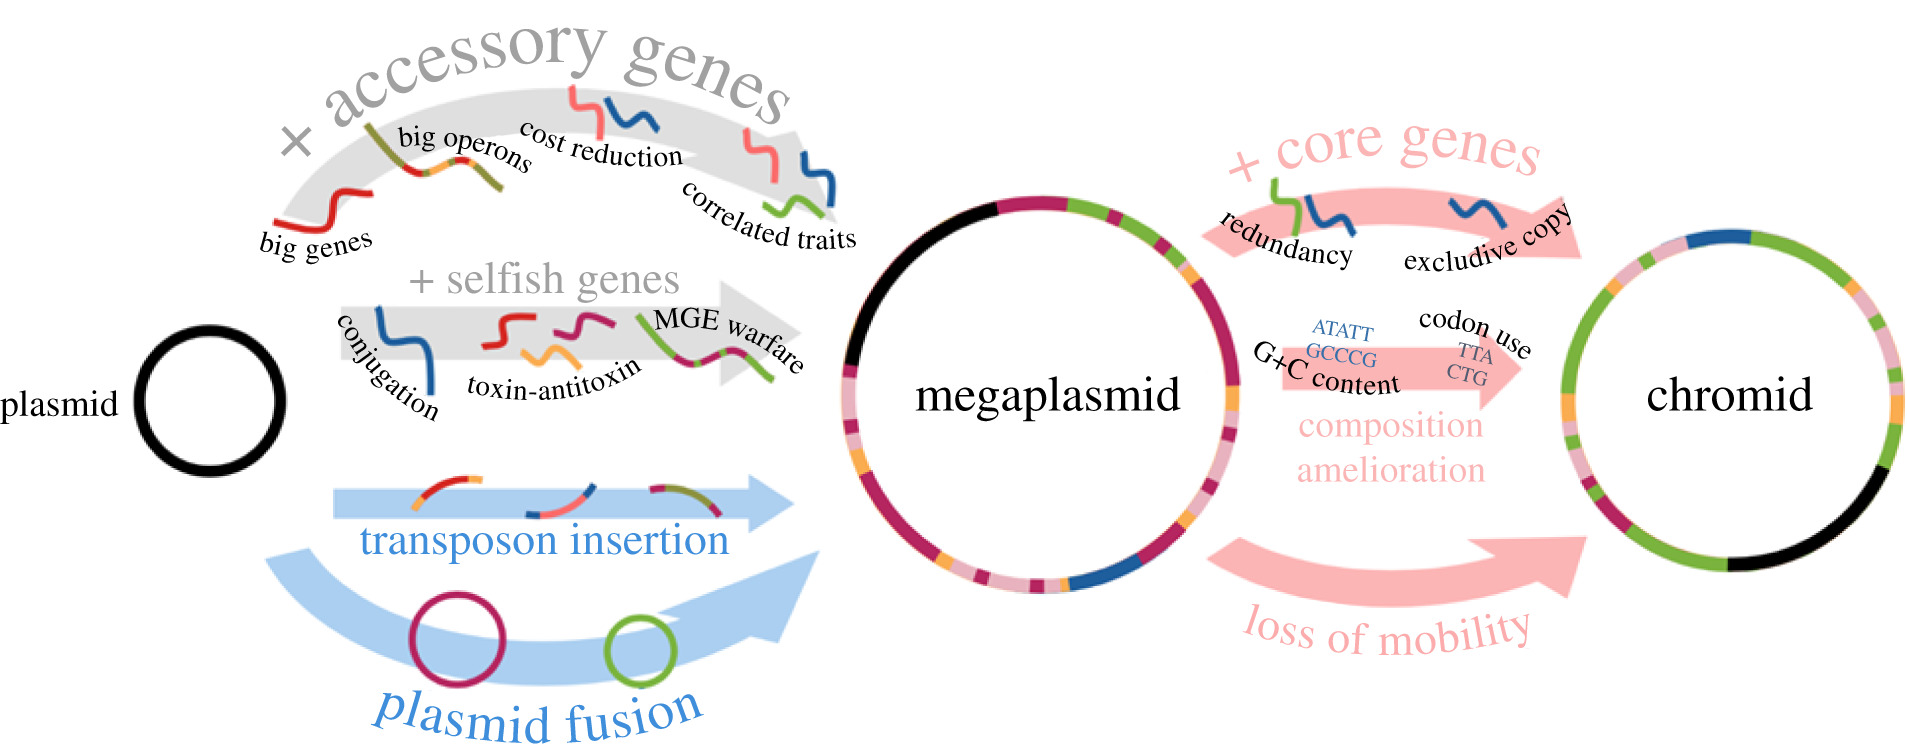
\includegraphics[width=.95\textwidth]{images/replicon.jpg}
    \caption[Évolution d'un plasmide en chromid]{\textbf{Schéma simplifié de l'évolution d'un plasmide en megaplasmide et de megaplasmide à chromide.} Figure extraite de \cite{hall_what_2021}}
    \label{fig:replicon}
\end{figure}

\newpage

Le génome procaryote correspond à l'ensemble des réplicons présents dans la cellule. La taille des génomes est comprise entre quelques centaines de milliers de bases à plusieurs millions de bases pour certains génomes\footnote{Un génome procaryote est compris entre 100 kb et 15 Mb. Pour comparaison, le génome humain mesure environs 3 Gb.} (\autoref{fig:genome_size}). Cette relative petite taille est optimisée par la structure des génomes et la proportion de séquence codante. Elle est aussi liée au mode de vie : les organismes endosymbiotiques ou pathogènes obligatoires, fortement dépendants de leur hôte, ont souvent un génome réduit en raison de la perte de gènes non essentiels. À l’inverse, les bactéries à vie libre possèdent généralement un génome plus large, leur permettant une plus grande autonomie métabolique et une meilleure adaptation aux variations environnementales.

\begin{figure}[htbp]
    \centering
    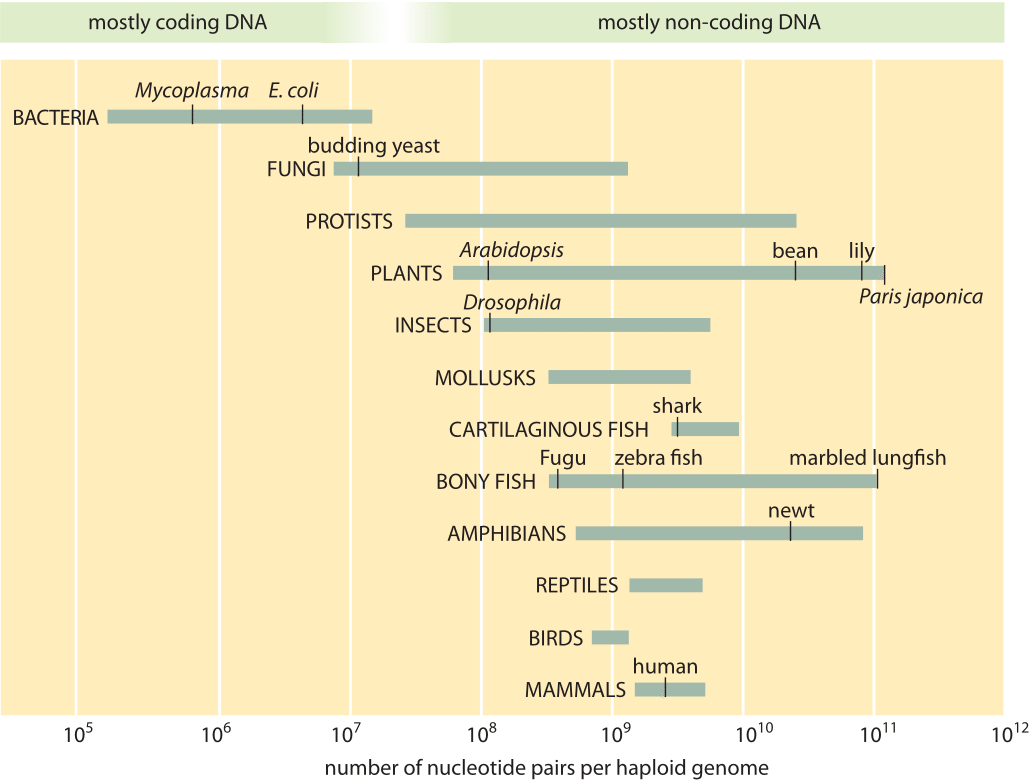
\includegraphics[width=\textwidth]{images/genome_size.png}
    \caption[Distribution de la taille des génomes chez les procaryotes]{\textbf{Distribution de la taille des génomes (en base) par classe chez les procaryotes.} Les données utilisées proviennent de RefSeq version 28 janvier 2025.}
    \label{fig:genome_size}
\end{figure}
